\subsubsection{2次元配列の例}

\Tchar 型の配列で作業していきます。これは、各要素がメモリ上に1バイトしか必要ないことを意味します。

\myparagraph{行を埋める例}
\myindex{\olly}

2行目を0~3の値で埋めてみましょう。

\lstinputlisting[caption=行を埋める例,style=customc]{patterns/13_arrays/5_multidimensional/two1_JA.c}

3つの行はすべて赤でマークしてあります。
2行目は0,1,2と3の値を持っています。

\begin{figure}[H]
\centering
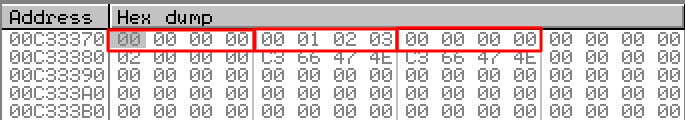
\includegraphics[width=0.6\textwidth]{patterns/13_arrays/5_multidimensional/olly_2D_1.png}
\caption{\olly: 配列が埋められる}
\end{figure}

\myparagraph{列を埋める例}
\myindex{\olly}

3列目を値0~2で埋めてみましょう。

\lstinputlisting[caption=列を埋める例,style=customc]{patterns/13_arrays/5_multidimensional/two2_JA.c}

3つの行はここでも赤でマークしてあります。

各行の3番目の値が0,1と2で書かれています。

\begin{figure}[H]
\centering
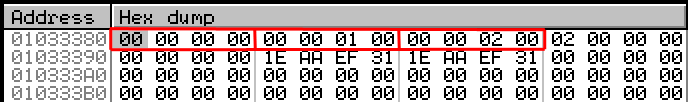
\includegraphics[width=0.6\textwidth]{patterns/13_arrays/5_multidimensional/olly_2D_2.png}
\caption{\olly: 配列が埋められる}
\end{figure}

